
%%%%%%%%%%%%%%%%%%%%%%%%%%%%%%%%%%%%%%%%%%%%%%%%%%%%%%%%%%%%%%%%%%%%%%%%%%%%%%%%%%
\begin{frame}[fragile]\frametitle{}
\begin{center}
{\Large Bayes Theorem Example}
\end{center}
\end{frame}


%%%%%%%%%%%%%%%%%%%%%%%%%%%%%%%%%%%%%%%%%%%%%%%%%%%%%%%%%%
\begin{frame}{Bayes Theorem  Example }

\begin{itemize}
\item  Suppose that $0.8\%$ of the general population has a certain disease, and suppose that we have a test for it.
\item The test says so $90\%$ of the time. 
\item If a person does not have the disease, the test gives a false diagnosis $7\%$ of the time. 
\item When a particular patient tests positive, what is the probability they have the disease?
\end{itemize}
\end{frame}

%%%%%%%%%%%%%%%%%%%%%%%%%%%%%%%%%%%%%%%%%%%%%%%%%%%%%%%%%%
\begin{frame}{Bayes Theorem  Example }

\begin{itemize}
\item   Let $D$ be the event that the person has the disease and $\bar{D}$ be its complement;
\item let $Y$ (for ``yes'') be the event that the test \emph{says} the person has the disease, with complement $\bar{Y}$.
\end{itemize}
\begin{eqnarray*}
	P(D)       &=& 0.008 \\
	P(Y|D)     &=& 0.90 \\
	P(Y|D\bar) &=& 0.07.
\end{eqnarray*}
\end{frame}

%%%%%%%%%%%%%%%%%%%%%%%%%%%%%%%%%%%%%%%%%%%%%%%%%%%%%%%%%%
\begin{frame}{Bayes Theorem  Example }

Let's find the probability
of $Y$ by itself.  Using the partition theorem we know this is
\begin{eqnarray*}
	P(Y) &=& P(Y|D)\,P(D) \;+\; P(Y|\bar{D})\,P(\bar{D}) \\
	&=& 0.90 \cdot 0.008 + 0.07\cdot 0.992 \\
	&=& 0.077.
\end{eqnarray*}
So the non-conditional probabilities are
\begin{align*}
	P(\bar{D})  &= 0.992  & P(\bar{Y})  &= 0.923 \\
	P(D)      &= 0.008  & P(Y)      &= 0.077.
\end{align*}
\end{frame}

%%%%%%%%%%%%%%%%%%%%%%%%%%%%%%%%%%%%%%%%%%%%%%%%%%%%%%%%%%
\begin{frame}{Bayes Theorem  Example }

\begin{itemize}
\item   Looking at $D$ and $Y$ separately, 
\item We can think of the population at large as
being split into those with and without the disease, and those for whom the
test is positive or negative.  
\item Suppose in particular that we have a sample of
1000 people who are representative of the general population. 
\end{itemize}
\end{frame}


%%%%%%%%%%%%%%%%%%%%%%%%%%%%%%%%%%%%%%%%%%%%%%%%%%%%%%%%%%
\begin{frame}{Bayes Theorem  Example }
Here are some
(very rectangular) Venn diagrams:
$$
%
	\begin{tabular}{|c|c||c|}
	\hline $\bar{D}$ & $D$ & \\
	\hline
	&&\\
	$992$ & $8$ & \\
	&&\\
	\hline
	\end{tabular}
%
	\qquad
	\qquad
%
	\begin{tabular}{|ccc||c|}
	\hline $\;$ & $\;$ & $\;$ & $\;$ \\
	\hline
	\hline  & &923& $\bar{Y}$ \\
	\hline  & & 77& $Y$ \\
	\hline
	\end{tabular}
%
$$
\end{frame}

%%%%%%%%%%%%%%%%%%%%%%%%%%%%%%%%%%%%%%%%%%%%%%%%%%%%%%%%%%
\begin{frame}{Bayes Theorem  Example }
Bayes' theorem has to do with how these two partitions intersect to make four
groups:
% $$
	\begin{tabular}{|r|r||c|}
	\hline $\bar{D}$ & $D$ & \\
	\hline
	\hline  $P(\bar{Y}|\bar{D}) \cdot 992 = ?$ & $P(\bar{Y}|D) \cdot 8 = ?$ & $\bar{Y}$ \\
	\hline  $P(Y    |\bar{D}) \cdot 992 = ?$ & $P(Y    |D) \cdot 8 = ?$ & $Y$ \\
	\hline
	\end{tabular}
%
	\qquad
	
	
	\textrm{and}
	
	
	\qquad
	
%
	\begin{tabular}{|r|r||c|}
	\hline $\bar{D}$ & $D$ & \\
	\hline
	\hline  $P(\bar{D}|\bar{Y}) \cdot 923 = ?$ & $P(D|\bar{Y}) \cdot 923 = ?$ & $\bar{Y}$ \\
	\hline  $P(\bar{D}|Y)     \cdot  77 = ?$ & $P(D|Y)     \cdot  77 = ?$ & $Y$ \\
	\hline
	\end{tabular}
% $$
\end{frame}




%%%%%%%%%%%%%%%%%%%%%%%%%%%%%%%%%%%%%%%%%%%%%%%%%%%%%%%%%%
\begin{frame}{Bayes Theorem  Example }
We can use the theorem to find the probability our patient has the
disease, given the positive test result:
\begin{eqnarray*}
	P(D|Y) &=& P(Y|D) \; \frac{P(D)}{P(Y)} \\
	&=& 0.90 \;\cdot\; \frac{0.008}{0.077} \\
	&=& 0.094.
\end{eqnarray*}
That is, there's only a one-in-eleven chance the patient actually has the
disease.
\end{frame}

%%%%%%%%%%%%%%%%%%%%%%%%%%%%%%%%%%%%%%%%%%%%%%%%%%%%%%%%%%
\begin{frame}{Bayes Theorem  Example }
We have two conditional probabilities given:  $P(Y|D)$ and $P(Y|\bar{D})$.  We
found $P(D|Y)$.  What about $P(D|\bar{Y})$?  We can use the  partition theorem
(theorem \ref{thm:partition}) again to solve for what we don't know in terms of
what we do know:
\begin{eqnarray*}
	P(D) &=& P(D|Y)\,P(Y) \;+\; P(D|\bar{Y})\,P(\bar{Y}) \\
	P(D|\bar{Y}) &=& \frac{P(D) - P(D|Y)\,P(Y)}{P(\bar{Y})} \\
	&=& \frac{0.008 - 0.094 \cdot 0.077}{0.923} \\
	&=& 0.0008.
\end{eqnarray*}
We now have all four conditional probabilities:
\begin{align*}
	P(Y|\bar{D}) &= 0.07  & P(D|\bar{Y}) &= 0.0008 \\
	P(Y|D)     &= 0.90  & P(D|Y)     &= 0.094.
\end{align*}
\end{frame}

%%%%%%%%%%%%%%%%%%%%%%%%%%%%%%%%%%%%%%%%%%%%%%%%%%%%%%%%%%
\begin{frame}{Bayes Theorem  Example }
Now we can fill out the four-square table:
\begin{itemize}

\item Since $P(Y|\bar{D})=0.07$, seven percent of the 992 disease-free people (70
of them) get false positives; the rest (922) get a correct negative result.

%These are the people in the left-hand column of the four-square table.

\item Since $P(Y|D)=0.90$, ninety percent of the 8 people with the disease test
positive (i.e. all but one of them); one of the 8 gets a false sense of security.

\item Since $P(D|\bar{Y})=0.0008$, $0.08\%$ of the 923 with negative test results
(one person) does in fact have the disease; the other 922 (as we found just above)
get a correct negative result.

\item Since $P(D|Y)=0.094$, only $9.4\%$ of the 77 people with positive test
results (7 people) have the disease; the other 70 get a scare (and, presumably,
a re-test).

\end{itemize}
\end{frame}

%%%%%%%%%%%%%%%%%%%%%%%%%%%%%%%%%%%%%%%%%%%%%%%%%%%%%%%%%%
\begin{frame}{Bayes Theorem  Example }
So, the sample of 1000 people splits up as follows:
$$
	\begin{tabular}{|r|r|c|}
	\hline $\bar{D}$ & $D$ & \\
	$922$ & $1$ & $\bar{Y}$ \\
	\hline  $70$ & $7$ & $Y$ \\
	\hline
	\end{tabular}
%
$$
Moreover, we can rank events by likelihood:
\begin{itemize}
\item[(1)] Healthy people correctly diagnosed: $92.2\%$.
\item[(2)] False positives: $7\%$.
\item[(3)] People with the disease, correctly diagnosed: $0.7\%$.
\item[(4)] False negatives: $0.1\%$.
\end{itemize}

Now it's no surprise our patient got a false positive:  this happens 10 times
as often as a correct positive diagnosis.
\end{frame}


% %%%%%%%%%%%%%%%%%%%%%%%%%%%%%%%%%%%%%%%%%%%%%%%%%%%%%%%%%%
% \begin{frame}
% \frametitle{Bayes Theorem}

% $P(\hbox{disease}|\hbox{positive})$\\
% \vspace{0.1in}


% \begin{equation*}=\frac{P(\hbox{disease})P(\hbox{positive}|\hbox{disease})}{P(\hbox{disease})P(\hbox{positive}|\hbox{disease})+P(\hbox{no disease})P(\hbox{positive}|\hbox{no disease})}\end{equation*}\\
% \vspace{.1in}

% \begin{equation*}
% =\frac{(0.05)(.92)}{(0.05)(0.92)+(0.95)(0.03)} \simeq 0.617\end{equation*}
% \end{frame}


%%%%%%%%%%%%%%%%%%%%%%%%%%%%%%%%%%%%%%%%%%%%%%%%%%%%%%%%%%%%
%%\begin{frame}{Bayes Theorem  Expanded}
%%
%%\begin{theorem} Let $A_1, A_2,\ldots,A_n$  be a set of mutually exclusive events that together  
%%form the sample space S. Let B be any event from the same sample space,  
%%such that $P(B) > 0$. Then, 
%%$$ P(A_k|B) = \frac{P(A_k \cap B)}{P(A_1 \cap B) + P(A_2 \cap B) + \ldots + P(A_n \cap B)}$$
%%$$ P(A_k|B) = \frac{P(A_k) P(B|A_k)}{P(A_1)P(B| \cap A_1) + \ldots + P(A_n)P( B|A_n)}$$
%%\end{theorem}
%%Note: The denominator in above equations is P(B).
%%\end{frame}
%%
%%%%%%%%%%%%%%%%%%%%%%%%%%%%%%%%%%%%%%%%%%%%%%%%%%%%%%%%%%%%
%%\begin{frame}{Bayes Theorem: Example  }
%% If a randomly selected lamp is defective, what is the probability that the 
%% lamp was manufactured in factory A3? 
%%\begin{center}
%%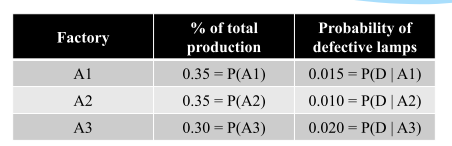
\includegraphics[width=0.8\linewidth,keepaspectratio]{bays1}
%%\end{center}
%%\end{frame}
%%
%%%%%%%%%%%%%%%%%%%%%%%%%%%%%%%%%%%%%%%%%%%%%%%%%%%%%%%%%%%%
%%\begin{frame}{Bayes Theorem: Example  }
%%\begin{center}
%%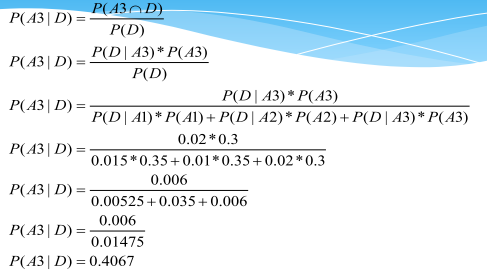
\includegraphics[width=0.8\linewidth,keepaspectratio]{bays2}
%%\end{center}
%%There is 40.67\% chance that, a defective product found is produced  
%%in Factory A3. 
%%\end{frame}
%%
%%%%%%%%%%%%%%%%%%%%%%%%%%%%%%%%%%%%%%%%%%%%%%%%%%%%%%%%%%
\begin{frame}{Comparisions}
\begin{itemize}\setlength{\itemsep}{0.3cm}

\item Classical statistics: model parameters are \emph{fixed} and \emph{unknown}.

\item A Bayesian thinks of parameters as random, and thus having distributions (just like the data). We can thus think about unknowns for which no reliable frequentist experiment exists, e.g. $\theta =$ proportion of US men with untreated prostate cancer.
		
\item A Bayesian writes down a \emph{prior} guess for parameter(s) $\theta$, say $p(\theta)$. He then combines this with the information provided by the observed data $by$ to obtain the \emph{posterior} distribution of $\theta$, which we denote by $p(\theta given by)$.

\item All statistical inferences (point and interval estimates, hypothesis tests) then follow from posterior summaries. For example, the posterior means/medians/modes offer point estimates of $\theta$, while the quantiles yield credible intervals.

\end{itemize}
\end{frame}

%%%%%%%%%%%%%%%%%%%%%%%%%%%%%%%%%%%%%%%%%%%%%%%%%%%%%%%%%%
\begin{frame}

\begin{itemize}\setlength{\itemsep}{0.5cm}
 \item The key to Bayesian inference is ``learning'' or ``updating'' of prior beliefs. Thus, posterior information $\geq$ prior information.

 \item Is the classical approach wrong? That may be a controversial statement, but it certainly is fair to say that the classical approach is limited in scope.

 \item The Bayesian approach expands the class of models and easily handles:
	\begin{itemize}
	\item repeated measures
	\item unbalanced or missing data
	\item nonhomogenous variances
	\item multivariate data
	\end{itemize}	
	-- and many other settings that are precluded (or much more complicated) in classical settings.
\end{itemize}

\end{frame}
